\documentclass[a4paper,12pt]{article}

% Comandos ---------------------------------------------------------------------
\setlength{\parindent}{1cm}
\newcommand{\mbf}[1]{\mathbf{#1}}
\let\D\displaystyle

% Margens ----------------------------------------------------------------------
\usepackage[top=3cm,left=3cm,right=2cm,bottom=2cm]{geometry}

% Pacotes Principais -----------------------------------------------------------
\usepackage[portuges,brazil]{babel}
\usepackage[utf8]{inputenc}

% Figuras e Imagens ------------------------------------------------------------
\usepackage{graphicx}
% Figuras lado a lado
\usepackage{epsfig}
\usepackage{subfigure}

% Utilizar H para inserir as imagens REALMENTE onde eu desejo
\usepackage{float}

% Fontes -----------------------------------------------------------------------
\usepackage[T1]{fontenc}
\usepackage{pslatex}

% Simbolos ---------------------------------------------------------------------
\usepackage{textcomp}
\usepackage{amsmath}

% Tabelas ----------------------------------------------------------------------
%\usepackage{multicol}
\usepackage{multirow}

% Comentários em bloco
\usepackage{verbatim}

% ------------------------------------------------------------------------------

\begin{document}
\begin{titlepage}
\begin{center}

\begin{table}[h]
\centering
\setlength{\arrayrulewidth}{3.5\arrayrulewidth}
    \begin{tabular}{cc}
    \hline\\
    \multirow{5}{*}{
\includegraphics[height=3cm]{imgs/ufrn}}&\\
    & \textsc{Universidade Federal do Rio Grande do Norte}\\
    & \textsc{Programa de P�s-Gradua��o em}\\
    & \textsc{Engenharia El�trica e de Computa��o}\\
    & \textsc{[EEC 2101] Controle Avan�ado}\\
    &\\
    &\\
    \hline
    \end{tabular}
\end{table}


\vfill

\LARGE
\textbf{1\textordfeminine\ Lista de Exerc�cios}

\vfill

\normalsize
\textbf{Anna Giselle C�mara Dantas Ribeiro}\\
\textbf{Cristiano Gurgel de Castro}\\
\textbf{Diogo Leite Rebou�as}\\
\textbf{Thiago Medeiros Barros}

\vfill
\textbf{Natal -- RN\\
        2010.1 }

\end{center}
\end{titlepage}


% ------------------------------------------------------------------------------
\section*{Questão 1}
% Enunciado
{\it Um sistema com realimentação unitária tem a seguinte função de
transferência de malha aberta:}

\begin{equation}\nonumber
G(s) = \frac{9}{s(s+p)}
\end{equation}

\noindent {\it em que $p$ é normalmente igual a 3. Determine a sensibilidade da
função de transferência de malha fechada $T(s)$ em relação ao parâmetro $p$ e
plote os diagramas de Bode (módulo e fase) para $p$ variando entre 1 e 5.
Analise os resultados.}

\vspace{0.5cm}

\noindent{\bf Resolução:}

\vspace{0.25cm}

\noindent Sabe-se que a função de transferência de malha fechada pode ser obtida
a partir da Eq. \ref{eq:G_MF}:

\begin{equation}\label{eq:G_MF}
G_{MF}(s) = \frac{G(s)}{1+G(s)H(s)}
\end{equation}

\noindent na qual $G(s)$ é função de transferência de malha aberta e $H(s)$ a
função de transferência do bloco da realimentação. Assim sendo, a função de
transferência de malha fechada para o sistema do enunciado com realimentação
unitária é dada por:

\begin{eqnarray}
G_{MF}(s) & = & \frac{G(s)}{1+G(s)H(s)}\nonumber\\
          & = & \frac{G(s)}{1+G(s)}\nonumber\\
          & = & \frac{\D\frac{9}{s(s+p)}}{1+\D\frac{9}{s(s+p)}}\nonumber\\
          & = & \frac{\D\frac{9}{s(s+p)}}{\D\frac{s(s+p)+9}{s(s+p)}}\nonumber\\
          & = & \frac{9}{s(s+p)+9}\nonumber\\
          & = & \frac{9}{s^2 + ps + 9}\label{eq:G_MF_q1}
\end{eqnarray}

A sensibilidade de um sistema é definida como sendo a razão entre a variação
percentual da função de transferência do sistema e a variação percentual da
função de transferência do processo (ou parâmetro). Ou seja, para uma dada
função de transferência do sistema $T(s)$, temos:

\begin{equation}
S = \frac{\Delta T(s)/T(s)}{\Delta G(s)/G(s)}
\end{equation}

No limite, para pequenas variações incrementais, temos:

\begin{equation}
S_G^T(s) = \frac{\partial T / T}{ \partial G / G} 
         = \frac{\partial T}{\partial G} \cdotp \frac{G}{T}
\end{equation}

Assim, para o parâmetro $p$ da função de transferência de malha fechada
obtida pela Eq. \ref{eq:G_MF_q1}, temos:

\begin{eqnarray}
S_p^G(s) & = & \frac{\partial G}{\partial p} \cdotp \frac{p}{G}\nonumber \\
         & = & \frac{0(s^2 + ps + 9) - 9(2s+p)}{(s^2 + ps + 9)^2} \cdotp
               \frac{p}{\D\frac{9}{s^2 + ps + 9}}\nonumber\\
         & = & - \frac{9(2s+p)}{s^2 + ps + 9} \cdotp \frac{p}{9}\nonumber\\
         & = & - \frac{2ps + p^2}{s^2 + ps + 9}
\end{eqnarray}

Substituindo $s$ por $j\omega$, temos:
\begin{equation}
S_p^G(j\omega) = - \frac{2pj\omega + p^2}{j\omega^2 + pj\omega + 9}
\end{equation}

Com $p = 1\text{,} 2\text{,} \ldots\text{,} 5$, obtém-se os diagramas de Bode
ilustrados pela Fig. \ref{fig:diag_bode_q1}.

\begin{figure}[htb]
\centering
    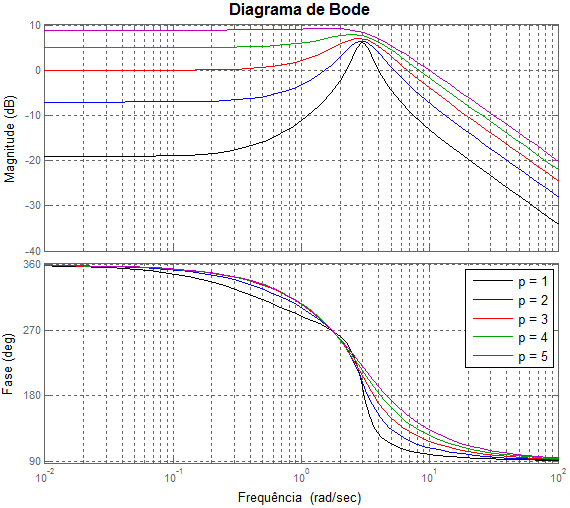
\includegraphics[width=0.8\textwidth]{imgs/questao1/bode}
    \caption{Diagrama de bode para $p = 1\text{,} 2\text{,} \ldots\text{,} 5$.}
    \label{fig:diag_bode_q1}
\end{figure}

Observa-se que para qualquer um dos valores de $p$, a função de transferência
possuirá polos complexos conjugados. Considerando a forma geral dos polos
complexos conjugados, dada pela Eq. \ref{eq:form_geral_polos_comp}, 

\begin{equation}\label{eq:form_geral_polos_comp}
S_p^G(j\omega) = 1 + 
                 \frac{2\zeta}{\omega_n}j\omega + 
                 \left(\frac{j\omega}{\omega_n}\right)^2
\end{equation}

\noindent percebe-se que, à medida que $\zeta$ decresce, as raízes em malha
fechada se aproximam do eixo imaginário e a resposta se torna cada vez mais
rápida (quanto ao tempo de subida) e oscilatória. Logo, aumentar o valor de $p$
leva a um aumento do fator de amortecimento $\zeta$, o que torna o sistema mais
lento.  Entretanto, essa “lentidão” é, de certa forma, compensada pelo ganho de
estabilidade, pois o sistema passa a ser menos oscilatório.

Observa-se ainda que o aumento do valor de $p$ leva a um aumento do ganho constante
do sistema, elevando a curva até aproximadamente 10dB para $p = 5$.

\pagebreak
% ------------------------------------------------------------------------------
\section*{Questão 2}
\pagebreak
% ------------------------------------------------------------------------------
\section*{Questão 3}
\pagebreak
% ------------------------------------------------------------------------------
\section*{Questão 4}


\end{document}
